\documentclass[../bericht.tex]{subfiles}

\begin{document}

  \chapter{Einleitung}

    Die Sekunde ist das $9.192.631.770$-fache der Periodendauer der dem Übergang zwischen den beiden Hyperfeinstrukturniveaus des Grundzustandes von Atomen des Nuklids $\mathrm{^{133}Cs}$ entsprechenden Strahlung - so die Definition nach dem SI-Einheitensystem. Genau diese Periodendauer soll im folgenden Versuch gemessen werden. Hierzu werden sowohl die Feinstruktur als auch die Hyperfeinstruktur erklärt und mittels der dopplerfreien Spektroskopie der Übergang aufgelöst.


  \chapter{Versuch}

    \section{Feinstruktur}
    \label{sec:feinstruktur}

      Nach dem semiklassischen Atommodell kreisen die negativ geladenen Elektronen auf einer Kreisbahn um den positiv geladenen Atomkern. Die Rotation stellt einen Kreisstrom dar. Dieser erzeugt ein magnetisches Dipolmoment, welches über den Bahndrehimpuls $\vec{l}$ ausgedrückt werden kann. Gemä\ss dem \textsc{Stern-Gerlach}-Experiment (und anderen Experimenten) haben Elektronen ein weiteres magnetisches Dipolmoment inne, welchem der Spin $\vec{s}$ zugrunde liegt. Die beiden magnetischen Momente wechselwirken in der sogenannten \textit{Spin-Bahn-Kopplung}. Je nach Einstellung des Elektronenspins (\textit{Spin-up}/ \textit{Spin-down}, d.h. für die $z$-Komponente des Spins $s_z=\pm \frac{\hslash}{2}$) ergibt sich eine positive, bzw. negative Energiekorrektur $\Delta E_{l,s}$, die sogenannte \textit{Spin-Bahn-Kopplungsenergie}.

      Bei der mathematischen Betrachtung sind für die \textit{Feinstrukturaufspaltung} außerdem relativistische Effekte zu beachten. Auf der Umlaufbahn um den ruhenden Kern dreht sich das Elektron einmal um die zum Drehimpuls parallele Achse. Dies führt zu einer Korrektur der kinetischen Energie $\Delta E_\mathrm{rel}$.

      Zuletzt muss der \textit{\textsc{Darwin}-Term} $\Delta E_\mathrm{Darwin}$ berücksichtigt werden. Als Folge der relativistischen Zitterbewegung des Elektrons auf seiner Kreisbahn verkompliziert sich die elektrostatische Wechselwirkung zwischen Elektron und Atomkern.
      \medskip

      Die gesamte Energiekorrektur
      \begin{equation*}
        \Delta E = \Delta E_{l,s} + \Delta E_\mathrm{rel} + \Delta E_\mathrm{Darwin}
      \end{equation*}
      führt zur sogenannten \textit{Feinstrukturaufspaltung}.
      \medskip

      Zur Beschreibung dieser Zustände wird der Gesamtdrehimpuls $\vec{j}=\vec{l}+\vec{s}$ mit der zugehörigen gutartigen Gesamtdrehimpulsquantenzahl $j$ eingeführt. Letzte kann die Werte
      \begin{equation*}
        j=+\frac{1}{2} \quad\text{für}\quad l=0
      \end{equation*}
      und
      \begin{equation*}
        j=l\pm \frac{1}{2}\quad\text{für}\quad l>0
      \end{equation*}
      annehmen. Somit spalten alle Zustände mit $l>0$ in zwei \textit{Feinstrukturniveaus} auf.


    \section{Hyperfeinstruktur}
    \label{sec:hyperfeinstruktur}

      Analog zum Spin des Elektrons wird auch dem räumlich ausgedehnten Atomkern ein Spin zugeordnet, der sogenannte \textit{Kernspin} $\vec{I}$. Das dem Spin zugeordnete magnetische Moment des Kerns wechselwirkt mit dem Gesamtspin des Elektrons $\vec{j}$. Wiederum kommt es je nach Ausrichtung des Kernspins zu einer Energiekorrektur welche positiv und negativ ausfallen kann. Die Projektion auf die $z$-Richtung von $\vec{I}$ kann die $(2I + 1)$ Werte
      \begin{equation*}
        I_z=m_I \cdot \hslash\quad\text{mit}\quad -I\le m_I \le +I
      \end{equation*}
      annehmen. Zur Zustandsbeschreibung wird nun der Gesamtdrehimpuls des Atoms $\vec{F}=\vec{j}+\vec{I}$ mit der zugehörigen gutartigen Quantenzahl $F$,
      \begin{equation*}
        |j-I| \le F\le |j + I|
      \end{equation*}
      eingeführt. Die \textit{Feinstrukturniveaus} spalten also in
      \begin{equation*}
        \begin{cases}
            (2I+1), & I<j\\
            (2j+1), & j<I
        \end{cases}
      \end{equation*}
      \textit{Hyperfeinstrukturniveaus} auf. Aufgrund der im Vergleich zum Elektron extrem großen Masse des Kerns
      \begin{equation*}
        m_\mathrm{Kern}\approx Z\cdot 1836 \cdot m_\mathrm{e},
      \end{equation*}
      mit der Kernladungszahl $Z$, ist die Energieaufspaltung in Folge der \textit{Hyperfeinstruktur} sehr klein. Um diese zu messen ist also extrem schmalbandiges Licht notwendig, welches gleichzeitig so intensiv sein muss, dass ein messbares Signal entsteht. Weil Monochromatoren zu breitbandig sind, erfordert das Experiment also einen Laser.


    \section{Termschema von Cäsium}
    \label{sec:termschema-caesium}

      Im Versuch wird das Nuklid $\mathrm{^{133}Cs}$ verwendet. Für die Zustände wird die Nomenklatur $n^{2s+1}l_j$  verwendet. Der relevante Teil des Termschemas von Cäsium für den Versuch, d.h. der Grundzustand $\mathrm{6^2 S_{1/2}}$ und der angeregte Zustand $\mathrm{6^2P_{3/2}}$ mit Feinstrukturaufspaltung und Hyperfeinstrukturaufspaltung sind in \cref{fig:feinstruktur-hyperfeinstruktur} abgebildet. Die Kernspinquantenzahl ist $I=\frac{7}{2}$. Weiter sind die erlaubten angeregten optischen Übergänge rot eingezeichnet. Für diese ist zu beachten, dass anregende Photonen einen Spin von $1$ tragen. Bei Verwendung von linear polarisiertem Licht gelten die Übergangsregeln
      \begin{equation*}
        \Delta l = 1\quad \text{und}\quad \Delta F = -1,0,+1.
      \end{equation*}

      \begin{figure}[tb]
        \centering
        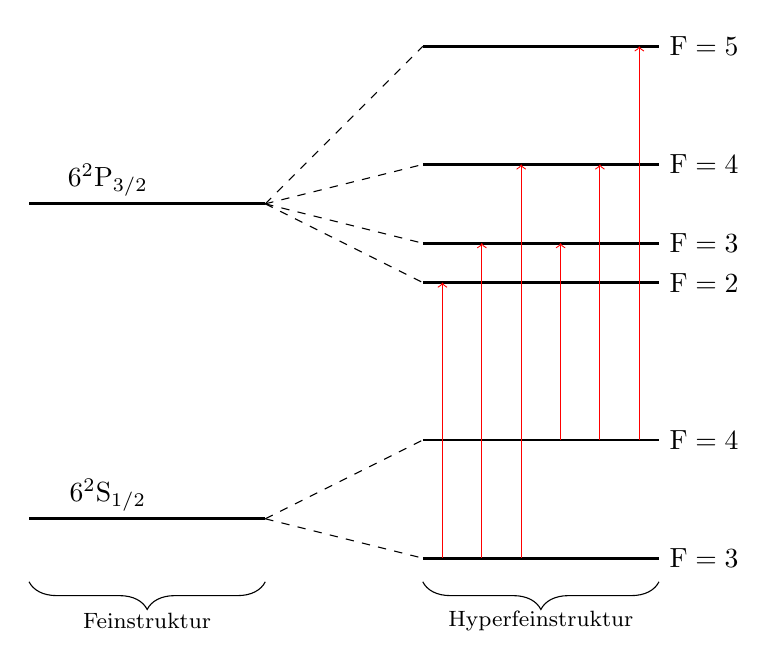
\begin{tikzpicture}
          % angeregte Niveaus
          \node at (1,4.3) {$\mathrm{6^2P_{3/2}}$};
          \draw[line width=1pt] (0,4)--(3,4);
          \draw[line width=1pt] (5,6)--(8,6) node[anchor=west] {$\mathrm{F=5}$};
          \draw[line width=1pt] (5,4.5)--(8,4.5) node[anchor=west] {$\mathrm{F=4}$};
          \draw[line width=1pt] (5,3.5)--(8,3.5) node[anchor=west] {$\mathrm{F=3}$};
          \draw[line width=1pt] (5,3)--(8,3) node[anchor=west] {$\mathrm{F=2}$};
          \draw[dashed] (3,4)--(5,6);
          \draw[dashed] (3,4)--(5,4.5);
          \draw[dashed] (3,4)--(5,3.5);
          \draw[dashed] (3,4)--(5,3);
          % Grundzustand Niveaus
          \node at (1,0.3) {$\mathrm{6^2S_{1/2}}$};
          \draw[line width=1pt](0,0)--(3,0);
          \draw[line width=1pt] (5,1)--(8,1) node[anchor=west] {$\mathrm{F=4}$};
          \draw[line width=1pt] (5,-0.5)--(8,-0.5) node[anchor=west] {$\mathrm{F=3}$};
          \draw[dashed] (3,0)--(5,1);
          \draw[dashed] (3,0)--(5,-0.5);
          % Übergänge
          % Unterer Grundzustand
          \draw[color=red, ->] (5.25,-0.5)--(5.25,3);
          \draw[color=red, ->] (5.75,-0.5)--(5.75,3.5);
          \draw[color=red, ->] (6.25,-0.5)--(6.25,4.5);
          % Oberer Grundzustand
          \draw[color=red, ->] (6.75,1)--(6.75,3.5);
          \draw[color=red, ->] (7.25,1)--(7.25,4.5);
          \draw[color=red, ->] (7.75,1)--(7.75,6);
          % Fein- und Hyperfeinstruktur
          \draw [decorate,decoration={brace,mirror,amplitude=10pt}] (0,-0.8) -- (3,-0.8) node [black,midway,yshift=-14pt] {\footnotesize Feinstruktur};
          \draw [decorate,decoration={brace,mirror,amplitude=10pt}] (5,-0.8) -- (8,-0.8) node [black,midway,yshift=-14pt] {\footnotesize Hyperfeinstruktur};
        \end{tikzpicture}
        \caption{Termschema von $\mathrm{^{133}Cs}$ ($I=\frac{7}{2}$) mit Feinstruktur und Hyperfeinstruktur. Die erlaubten Anregungsübergänge sind rot markiert. }
        \label{fig:feinstruktur-hyperfeinstruktur}
      \end{figure}


    \section{Diodenlaser}
    \label{sec:diodenlaser}

      Es folgt eine Kurzfassung von ??? zur Funktion von Diodenlasern.

      Diodenlaser sind aus Halbleitern aufgebaut. Bei der Rekombination von Elektronen im Leitungsband mit den Löchern im Valenzband wird das Laserlicht emittiert. Der Hauptteil eines Diodenlasers besteht aus einem $p-n$-Übergang, welcher durch Dotierung erzeugt wird. Die Besetzungsinversion mit Löchern im Valenzband und Elektronen im Leitungsband wird durch das Anlegen einer Spannung erreicht. Dieser Prozess ist der Pumpprozess des Lasers. Die Rekombination der Löcher und Elektronen kann spontan oder stimuliert erfolgen. Das dabei emittierte Licht ist nur kohärent, falls die stimulierte Emission überwiegt. Aufgrund des hohen Brechungsindexes $n$ der Halbleiterkristalle beträgt die Reflektivität der Grenzfläche zu Vakuum in etwa $\SI{30}{\percent}$. Damit können die Kristalle selbst, ohne weitere Behandlung, als Resonatoren fungieren. Diejenige Seite, auf der kein Licht austreten soll, wird zusätzlich verspiegelt. Für die Ausbildung von stehenden Wellen im Resonator gilt der Zusammenhang
      \begin{equation*}
        \lambda = \frac{2nL}{m}.
      \end{equation*}
      Hierbei ist $\lambda$ die Wellenlänge des Lichts, $L$ die Länge des Resonators (Halbleiterkristalls) und $m$ eine natürliche Zahl.

      Einer der Vorteile eines Diodenlasers ist dessen Durchstimmbarkeit bezüglich der Frequenzen. In Abhängigkeit der Betriebstemperatur $T$ und der Stromstärke $I$ ??? ändert sich die Frequenz der Laserstrahlung. Die Temperatur beeinflusst die Ausdehnung des Kristalls und damit die Länge des Resonators. Unter Voraussetzung einer konstanten Temperatur ändert sich mit der Stromstärke die Ladungsträgerdichte im Halbleiter. Damit ändert sich auch der Brechungsindex des Kristalls und somit die optische Länge des Resonators.
      Die Durchstimmbarkeit ist für diesen Versuch von Bedeutung, um die Resonanzfrequenz von Cäsium zu treffen.

      Die Laserschwelle des in diesem Versuch verwendeten Lasers liegt bei.... ????

      Weiter weist ein Diodenlaser, wie alle Laser, eine schmale Linienbreite auf, welche nötig ist um die Energieaufspaltung der Hyperfeinstruktur auflösen zu können. Das Spektrum des verwendeten Lasers ist in ??? abgebildet. Dieses ist jedoch noch immer zu breit für die gewünschte Auflösung der Hyperfeinstruktur. Die Linienbreite des Lasers erscheint verbreitert durch die \textit{natürliche Linienbreite}, \textit{\textsc{Doppler}verbreiterung} und \textit{Druckverbreiterung}. Dominant ist hierbei die \textit{\textsc{Doppler}verbreiterung}, wie in folgenden Abschnitten erläutert wird. Deshalb folgt auch die Notwendigkeit der \textit{\textsc{doppler}freien Spektroskopie} (vgl. \ref{sec:dopplerfreie-spektroskopie}).


      \subsection{Druckverbreiterung}
      \label{subsec:druckverbreiterung}

        Je nach Gasdruck in der Gaskammer kommt es zu mehr oder weniger Stößen zwischen den
        Cäsium-Atomen. Die Wechselwirkung zwischen den Atomen beeinflusst das Termschema und
        verbreitert damit die Spektrallinien. Die Linienverbreiterung ist proportional zum Druck. Somit kann und wird der Effekt der \textit{Druckverbreiterung} durch einen kleinen Druck in der Gaskammer minimiert.


      \subsection{Natürliche Linienbreite}
      \label{subsec:natueliche-linienbreite}

        Angeregte Zustände haben nur eine endliche Lebensdauer bevor das System wieder in den Grundzustand relaxiert. Nach der \textit{\textsc{Heisenberg}'schen Unschärferelation} können Zeit und Energie aber nicht gleichzeitig scharf bestimmt werden. Somit gehören zu Zuständen mit begrenzter Lebensdauer unscharfe Energieniveaus. Dies sorgt für eine Verbreiterung der Spektrallinien. Die Unschärfe aufgrund der sogenannten \textit{natürlichen Linienbreite} ist allerdings für die optischen Cäsium Übergänge, welche in diesem Versuch von Interesse sind, hinreichend klein um die Hyperfeinstruktur auflösen zu können.


      \subsection{Dopplerverbreiterung}
      \label{subsec:dopplerverbreiterung}

        Gemä\ss dem relativistischen \textsc{Doppler}-Effekt ändert sich die Frequenz eines einfallenden Photons im Ruhesystem eines (Cäsium-) Atoms, falls das Atom eine Geschwindigkeitskomponente ungleich Null parallel zur Bahn des Photons aufweist. Im Falle von entgegengesetzten Bewegungen von Atom und Photon kommt es zur Blauverschiebung (die vom Atom observierte Frequenz wird größer), im Falle von gleichgerichteten Bewegungen zur Rotverschiebung (die vom Atom observierte Frequenz wird kleiner). Mit dem \textsc{Doppler}-Effekt als Ursache wird diese Linienverbreiterung \textit{\textsc{Doppler}verbreiterung} genannt.


    \section{Transmissionsspektroskopie}
    \label{sec:transmissionsspektroskopie}




    \section{Dopplerfreie Spektroskopie}
    \label{sec:dopplerfreie-spektroskopie}


      6 statt 3 erwartete Peaks


      \subsection{Cross-over Resonanzen}
      \label{subsec:cross-over-resonanzen}

        genau in der mittels


    \section{Zeeman-Effekt}
    \label{sec:zeeman-effekt}

      nicht observierbar!










\end{document}
